\documentclass{article}
\usepackage[utf8]{inputenc}
\usepackage{graphicx}
\usepackage{epstopdf}
\usepackage{float}
\usepackage[margin=1.25in]{geometry}
\usepackage{amsmath}
\usepackage{amssymb}
\usepackage{color} 
\usepackage{fancyvrb} 
\newcommand{\Vb}{{$V_{b}$}}
\newcommand{\Vtwo}{{$V_{2}$}}
\newcommand{\Vone}{{$V_{1}$}}
\newcommand{\Itwo}{{$I_{2}$}}
\newcommand{\Ione}{{$I_{1}$}}
\newcommand{\Vdd}{{$V_{dd}$}}
\newcommand{\Iout}{{$I_{out}$}}
\newcommand{\gm}{{$g_{m}$}}
\newcommand{\Vdm}{{$V_{dm}$}}
\newcommand{\Idm}{{$I_{dm}$}}
\newcommand{\Icm}{{$I_{cm}$}}
\newcommand{\Ib}{{$I_{b}$}}
\newcommand{\nMOS}{{\textit{n}MOS }}
\newcommand{\pMOS}{{\textit{p}MOS }}
\title{Circuits Lab 8}
\author{Cory Dolphin and Noam Rubin}
\date{April 14, 2013}

\begin{document}

\maketitle

\section*{Experiment 1}

\begin{figure}[H]
\centering
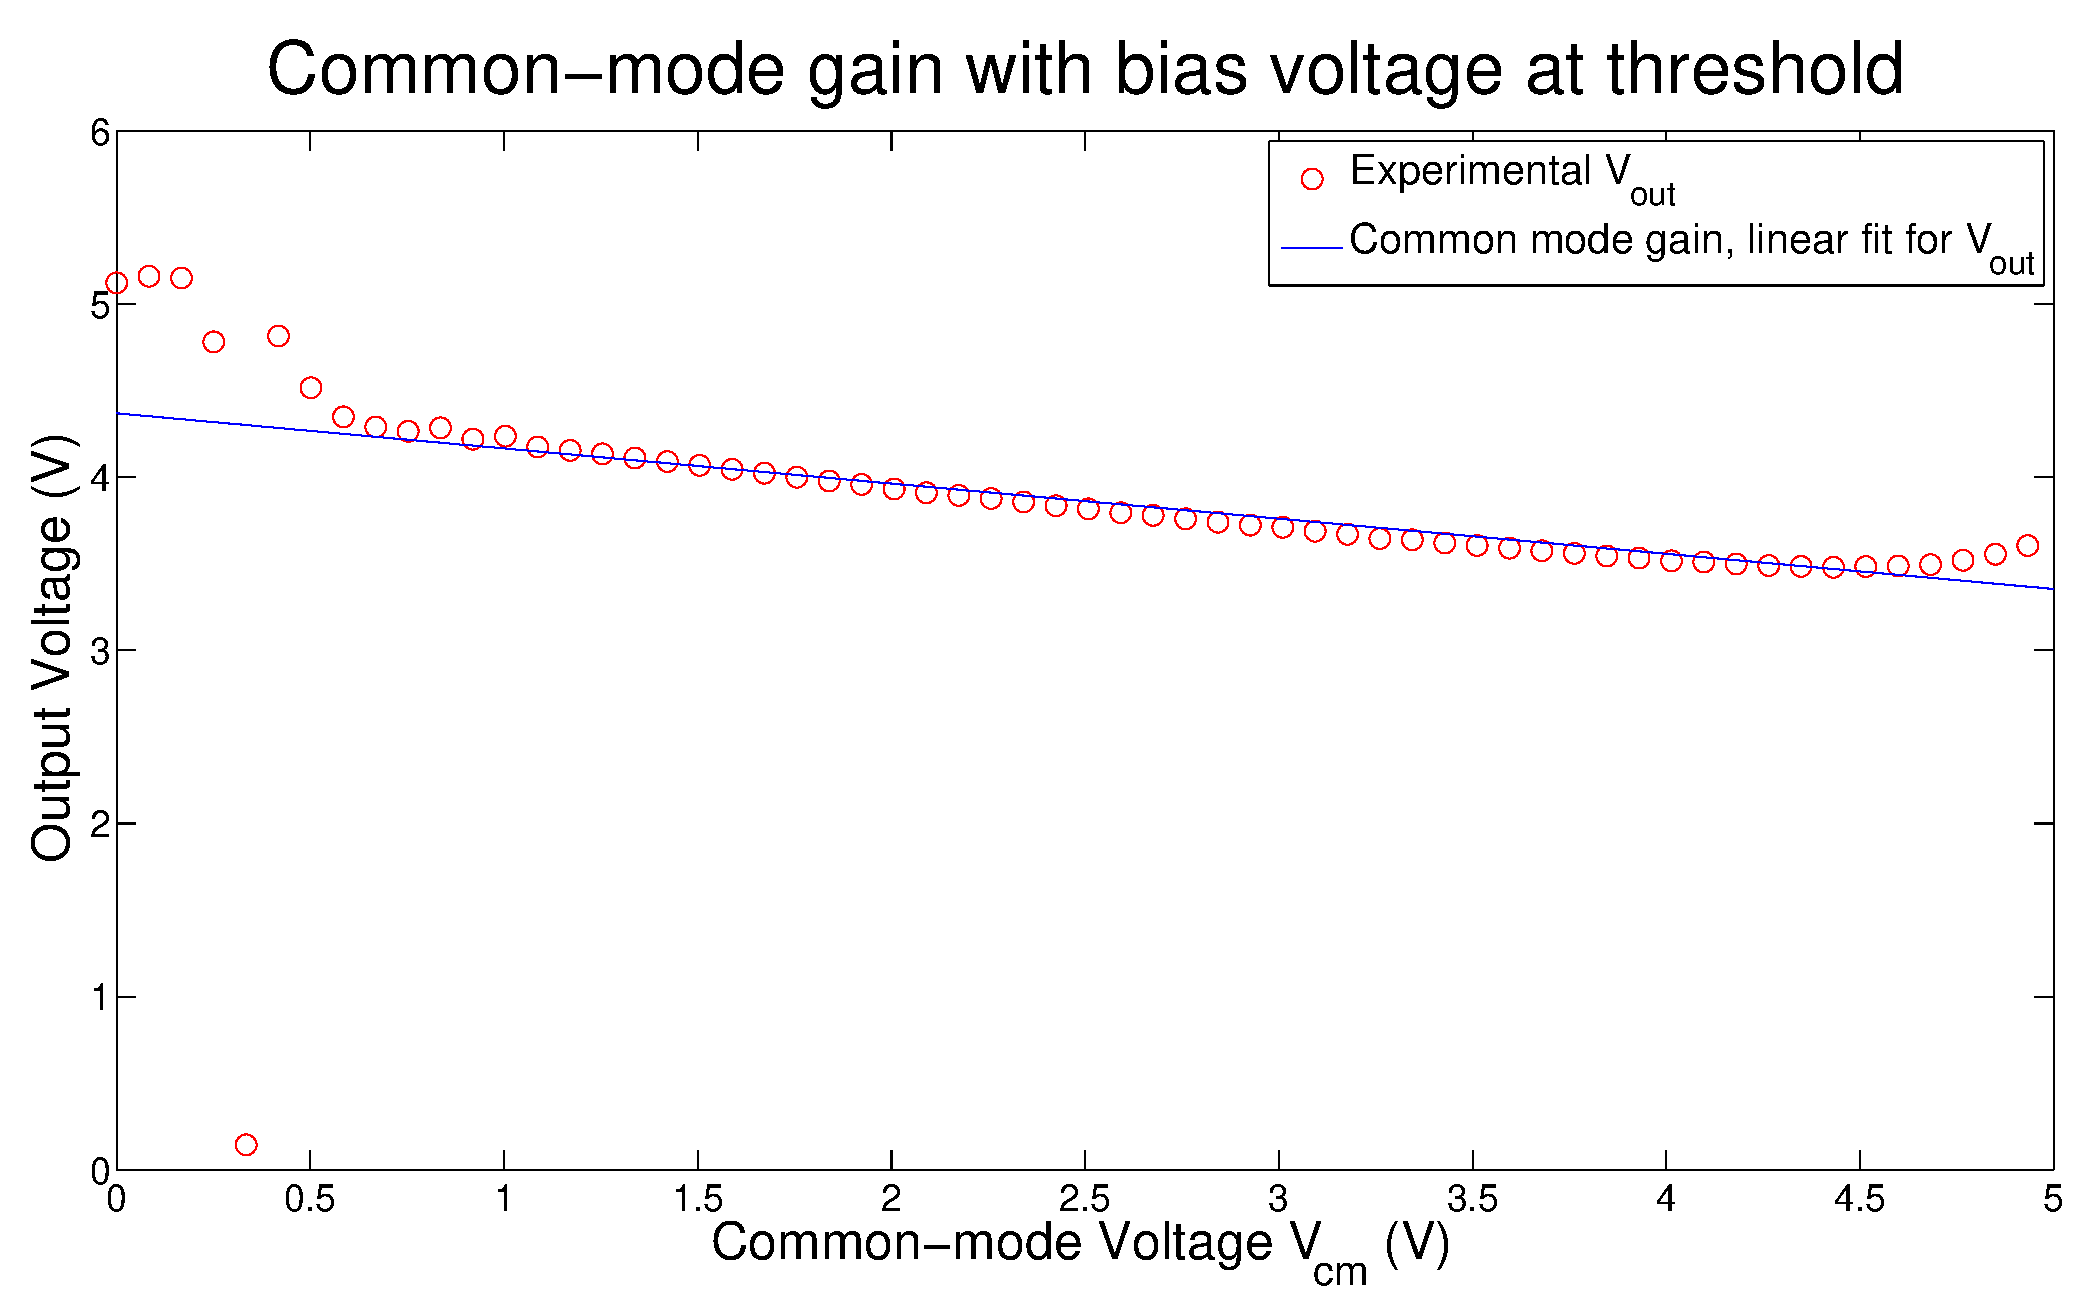
\includegraphics[width=\linewidth]{../Figures/Exp1P1.eps}
\caption{Something descriptive..}
\label{fig:exp1p1}
\end{figure}

\begin{figure}[H]
\centering
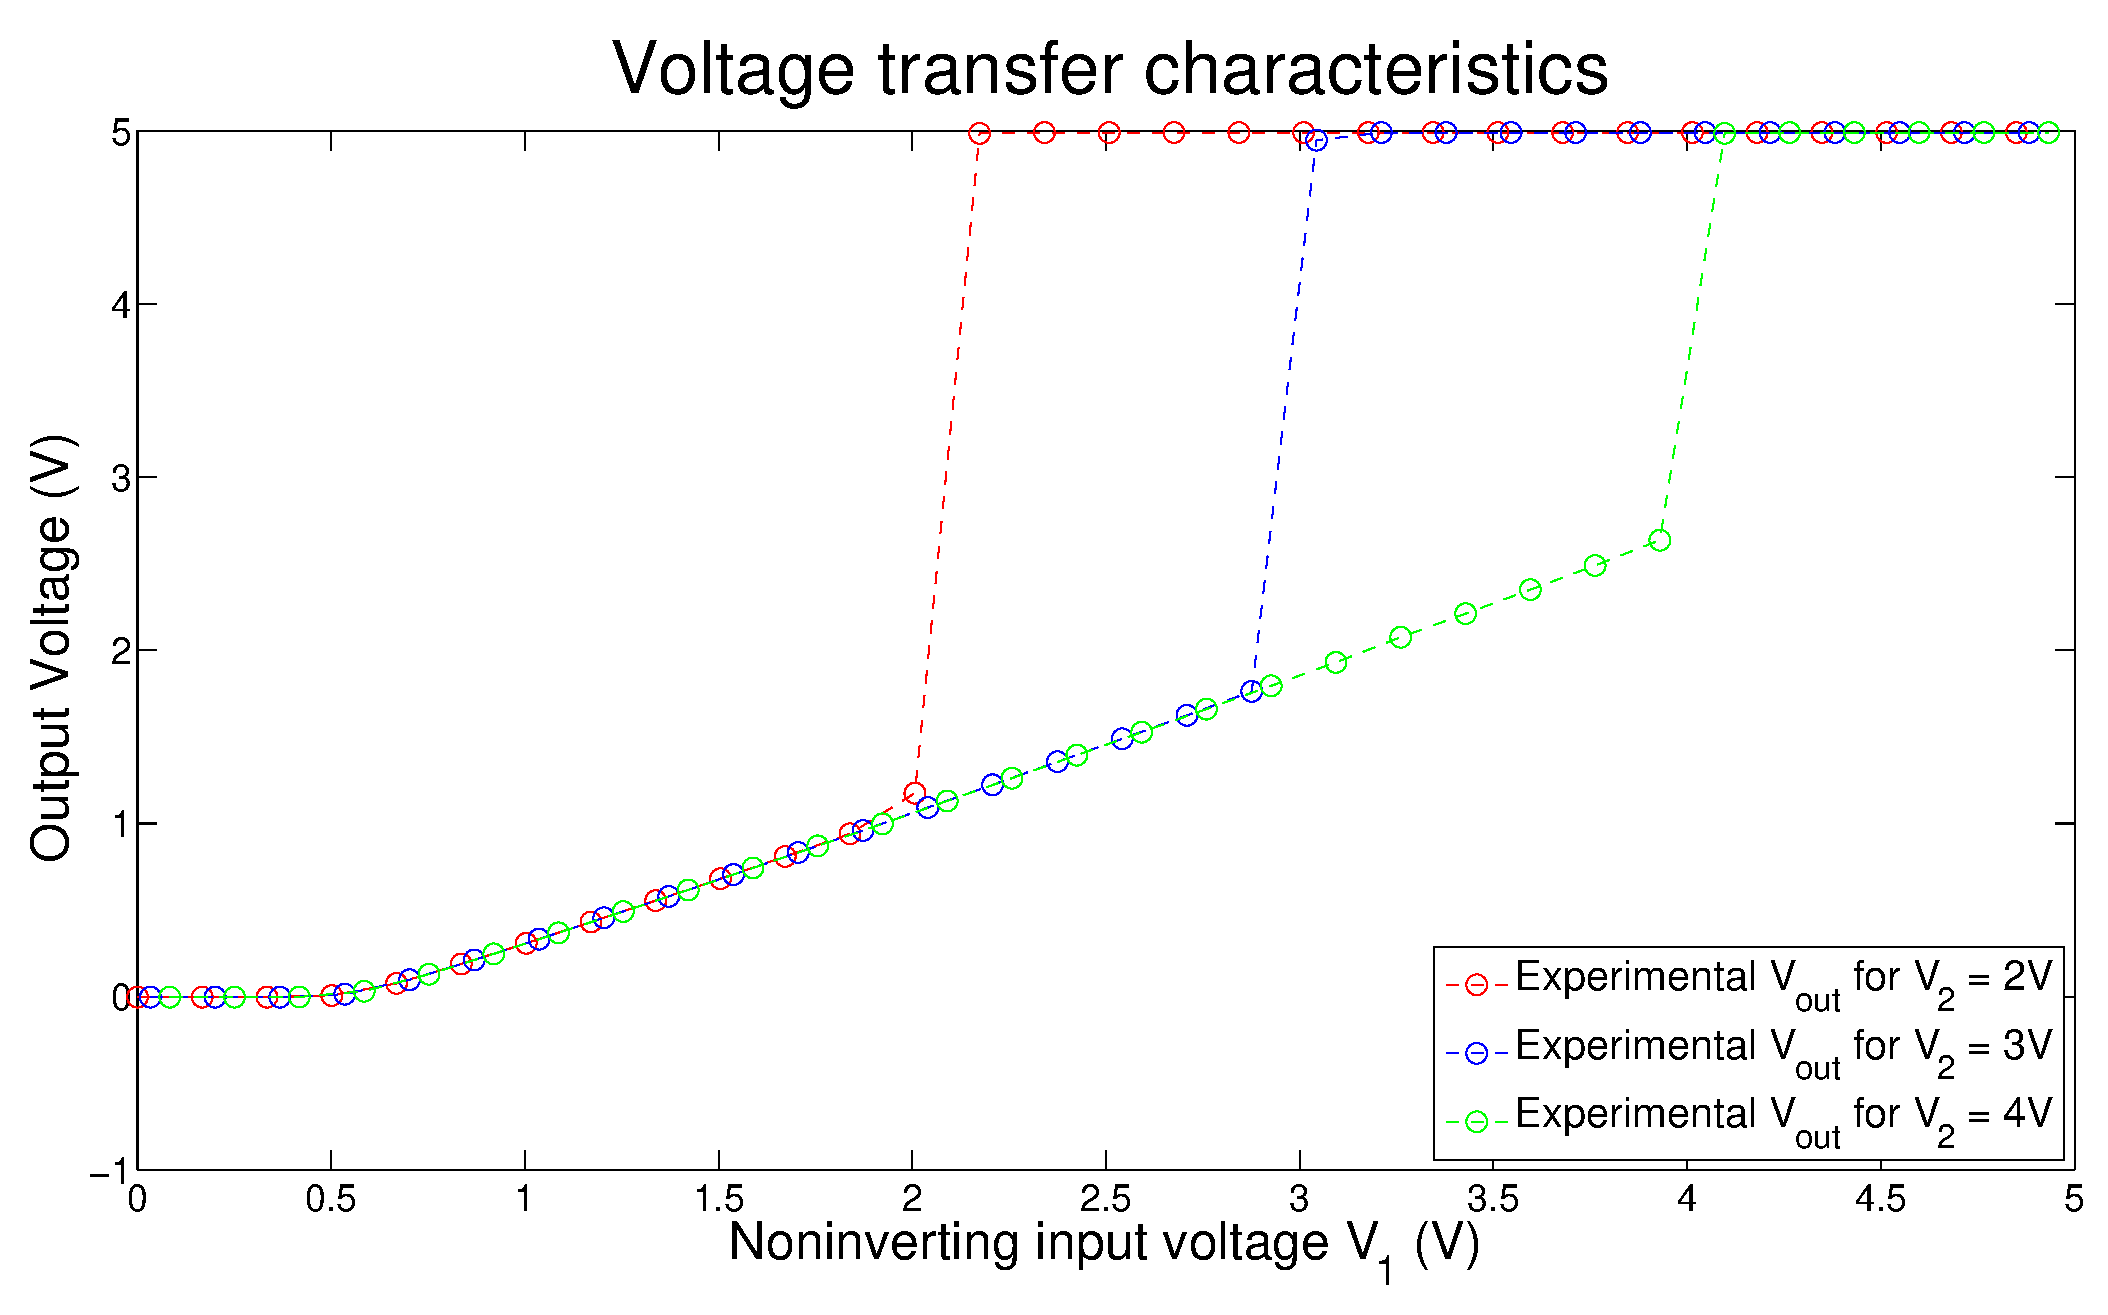
\includegraphics[width=\linewidth]{../Figures/Exp1P2.eps}
\caption{Something descriptive..}
\label{fig:exp1p2}
\end{figure}

\section*{Experiment 2}

\section*{Experiment 3} 

\begin{figure}[H]
\centering
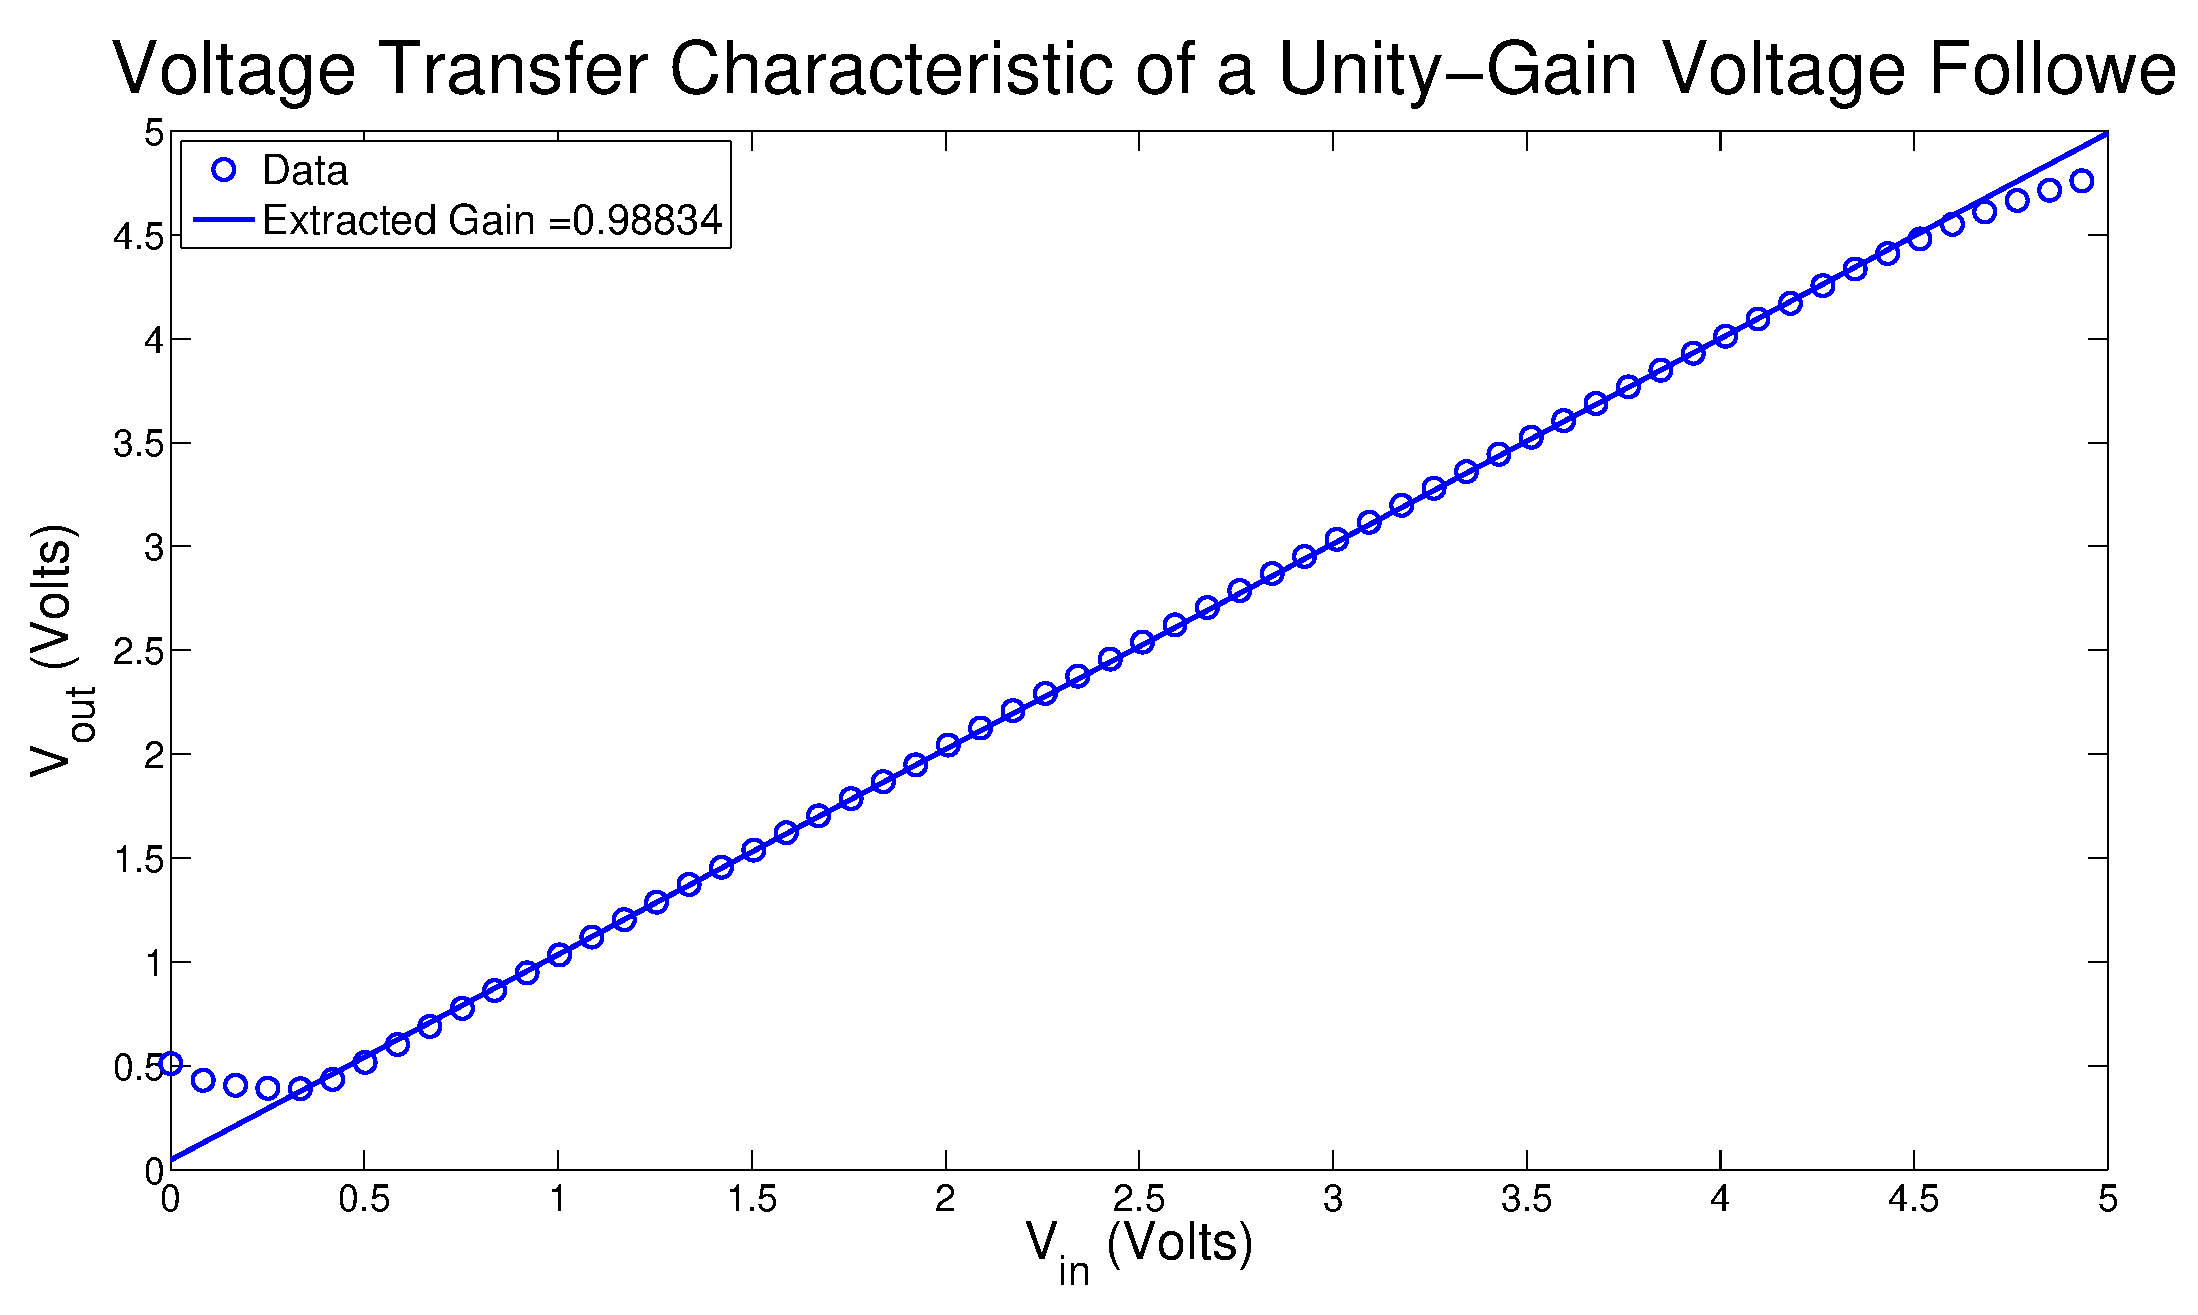
\includegraphics[width=\linewidth]{../Figures/Exp3P1.eps}
\caption{Something descriptive..}
\label{fig:exp3p1}
\end{figure}

\begin{figure}[H]
\centering
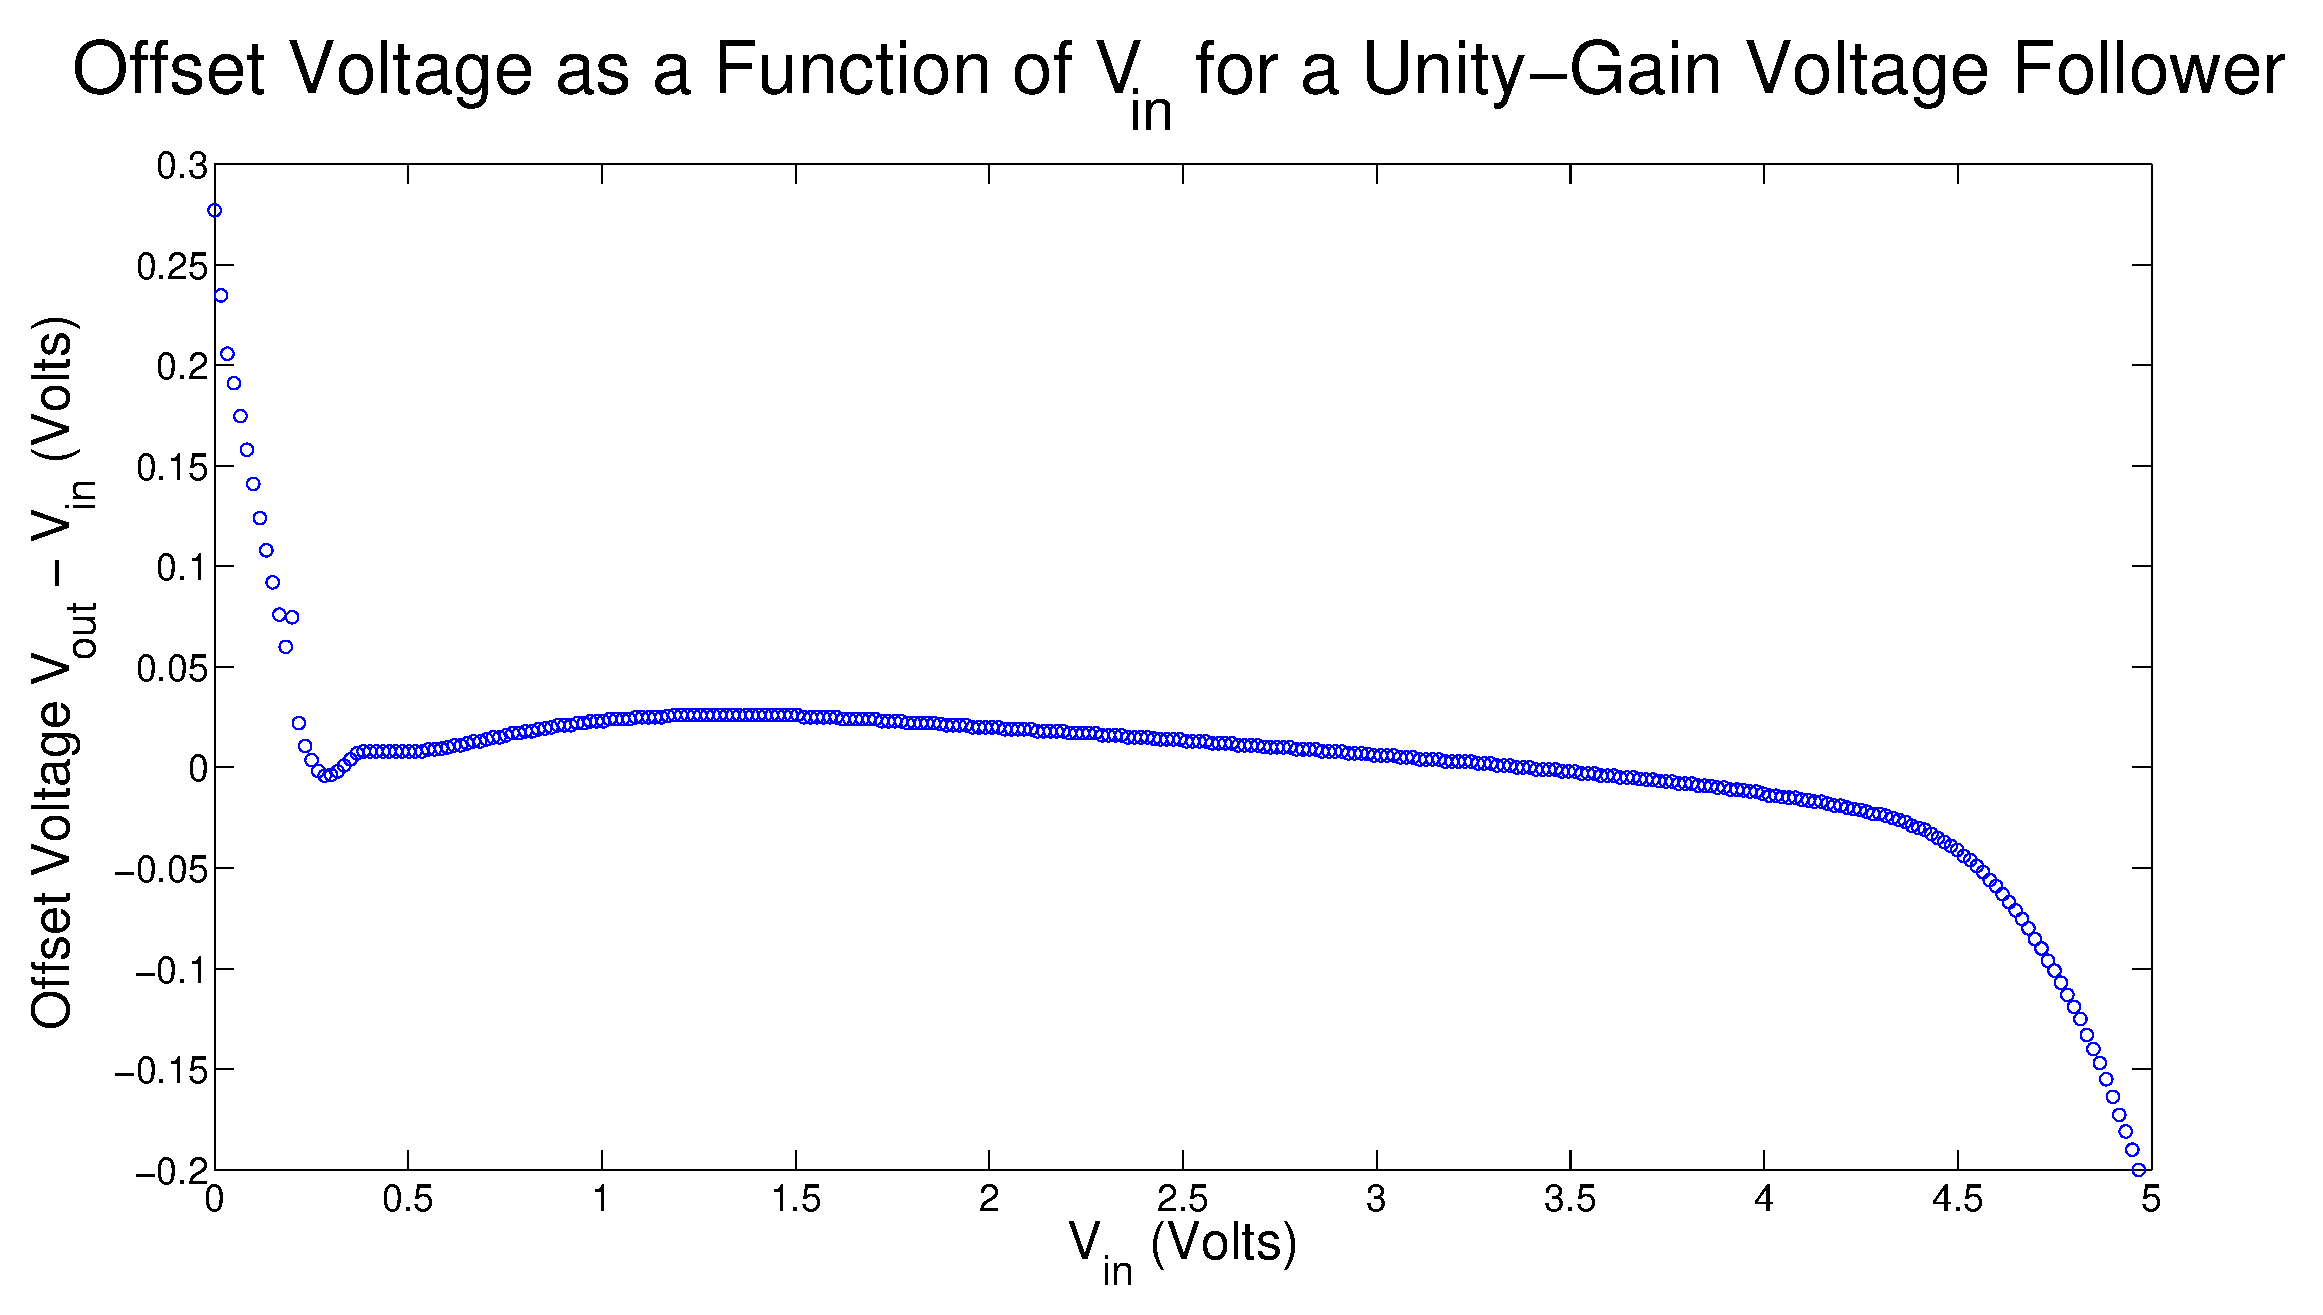
\includegraphics[width=\linewidth]{../Figures/Exp3P2.eps}
\caption{Something descriptive..}
\label{fig:exp3p2}
\end{figure}





\end{document}